\documentclass[a4paper]{report}
\usepackage{amsmath,amssymb,booktabs,bm,caption,enumerate,float,geometry,graphicx,hanging,indentfirst,makecell,multirow,setspace,titlesec}
\geometry{left=4.5cm,right=4.5cm,top=4cm,bottom=4cm}
\captionsetup[figure]{labelsep=period}
\captionsetup[table]{labelsep=period}
\begin{document}
	\renewcommand\thesection{\arabic{section}}
	\begin{Large}
		\begin{center}
			\setlength{\baselineskip}{14pt}
			\vspace{1.25cm}
			\rule[0cm]{11.2cm}{0.03em}\\
			\vspace{0.5cm}
			\textsc{UM-SJTU Joint Institute}\\
			\vspace{0.25cm}
			\textsc{Intro to circuits\\(VE215)}
			\vspace{0.3cm}
			\rule[0cm]{11.8cm}{0.05em}
			\vspace{4.9cm}\\
			\textsc{Laboratory Report}
		\end{center}
	\end{Large}
	\vspace{0.85cm}
	\begin{large}
		\begin{center}
			\textsc{Lab 4}
			\vspace{1em}\\
			\textsc{AC Lab}
		\end{center}
		\vspace{6cm}
	\end{large}
	\begin{tabular}{l l}
	Name: Yihua Liu&ID: 518021910998\\
	Name: Han Fang&ID: 518370910009\\
	Name: Yiteng Cai&ID: 518370910007\\
	&\\
	Date: \today&\\
	\end{tabular}
	\thispagestyle{empty}
	\newpage
\section{Introduction}
\subsection{Objectives}
\begin{enumerate}
	\item Learn how to define, calculate, and measure the amplitude of a sinusoidal signal
	\item Learn how to define, calculate, and measure the Rise Time and Fall Time of a signal
	\item Learn how to observe FFT spectra of signal and measure their parameters with cursors
	\item Measure the waveforms and FFT spectra of various signals
	\item Compare your theoretical results obtained in the Pre-Lab with your In-Lab data.
\end{enumerate}
\section{Introduction}
\subsection{High-Z mode}
We have already learnt Thevenin equivalent of a circuit. You can think the function generator in terms of its Thevenin equivalent circuit, which includes the voltage source and $V_S$ and the equivalent resistance of 50 $\Omega$ as shown below.
\begin{figure}[H]
	\centering
	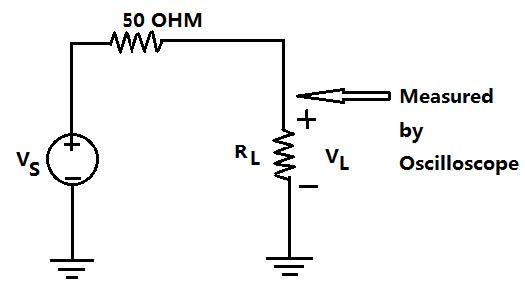
\includegraphics[width=10cm]{1.jpg}
\end{figure}
When the load $R_L$ is 50 $\Omega$ , according to voltage division, we know that the $V_L$ measured will be 0.5$V_S$. In this case, we use the 50 OHM mode, in which the function generator produces voltage $V_S$ but displays voltage 0.5$V_S$. In that way, if you set 2$V_{\rm{ppk}}$ for the function generator, the actual $V_S$ will be 4$V_{\rm{ppk}}$ to make sure the load get a voltage of 2$V_{\rm{ppk}}$.

In our lab measurements, the load resistance $R_L$ is very high—the input resistance of the oscilloscope is about 1 $M\Omega$ . The $V_L$ measured across $R_L$ practically equals $V_S$. So we use High Z mode, in which the function generator produce voltage $V_S$ and displays $V_S$.
\subsection{The Rise Time and Fall Time of signals}

The Rise time is the interval between the moment of the time when the signal reaches its 10\% level and the moment of time when the signal reaches its 90\%. We have already used this concept in our Lab3.
\begin{figure}[H]
	\centering
	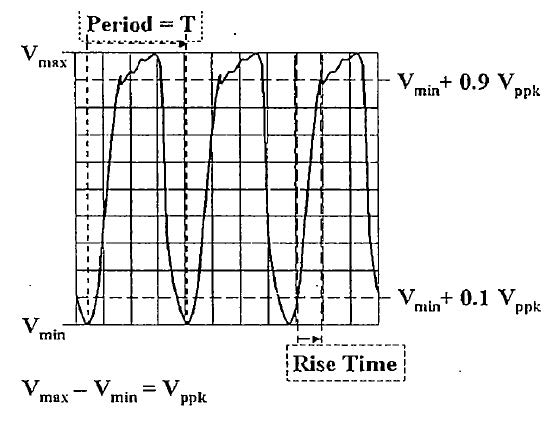
\includegraphics[width=10cm]{2.jpg}
\end{figure}
\begin{figure}[H]
	\centering
	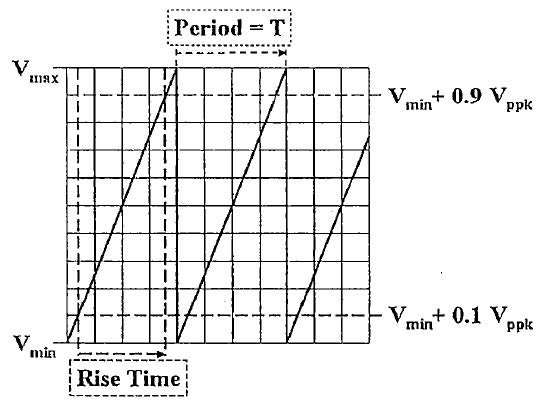
\includegraphics[width=10cm]{3.jpg}
\end{figure}
The above two figures illustrate the rise time of a sinusoidal like wave and a saw-tooth wave. If you do not know what is $V_{\rm{ppk}}$, we can refer to part 4 of this section.

Take the sinusoid wave as an example to calculate the rise time.
$$y=\frac{V_{\rm{ppk}}}{2}\sin(2\pi ft)$$
$$V_{min}=\frac{-V_{\rm{ppk}}}{2},V_{max}=\frac{V_{\rm{ppk}}}{2}$$
$$\mathrm{Rise\ Time}=\frac{\sin^{-1}\left(\frac{V_{min}+0.9V_{\rm{ppk}}}{0.5V_{\rm{ppk}}}\right)-\arcsin^{-1}\left(\frac{V_{min}+0.1V_{\rm{ppk}}}{0.5V_{\rm{ppk}}}\right)}{2\pi f}$$
\subsection{Fourier Series Representation of a Signal}

We will learn Fourier Series in details in our math course this semester.

Fourier series is a way to represent a wave-like function as a combination of simply sine waves. It decomposed and period function into the sum of a (possibly infinite) set of simple oscillation functions.

Let $x(t)$ be a periodic signal with fundamental period $T_0$. It can be represent by the following synthesis equation,
$$x(t)=\sum_{k=-\infty}^{\infty}c_ke^{jk\omega_0t}\ ,\mathrm{where}\ \omega_0=\frac{2\pi}{T_0}$$
The coefficients $c_k$ in the above equation can be calculated by the analysis
equation,
$$C_k=\frac{1}{T_0}\int_0^{T_0}x(t)e^{-jk\omega_0t}dt,k=0,\pm 1,...$$

Plot[Sum[(-1)\^((($k$ + 1))/2) * 2/(($k$ * Pi) ) Cos[$k$ * Pi * ($t$ +0.5)], {$k$, 1,100,2}], {$t$, -4,4}]

We can use the above Mathematica code to get the feeling of how a series of sinusoidal waves can form a square wave (actually, any waveform). We can change the value in the red box, and the larger the value is, the more accurate the result will be.

For value 3, we can get the following result.
\begin{figure}[H]
	\centering
	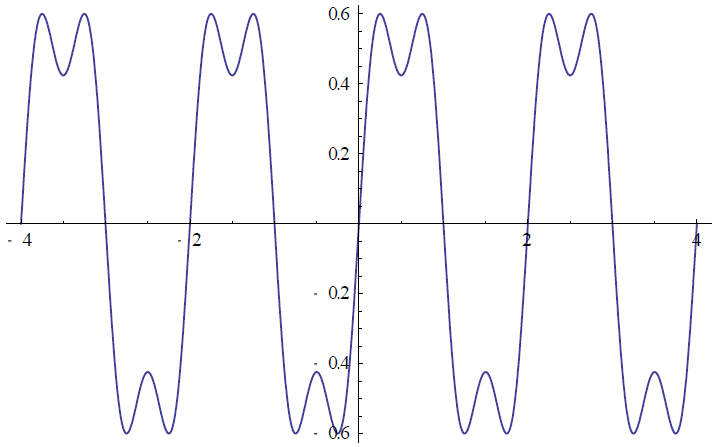
\includegraphics[width=1\linewidth]{4.png}
\end{figure}
For value 20, we can get the following result,
\begin{figure}[H]
	\centering
	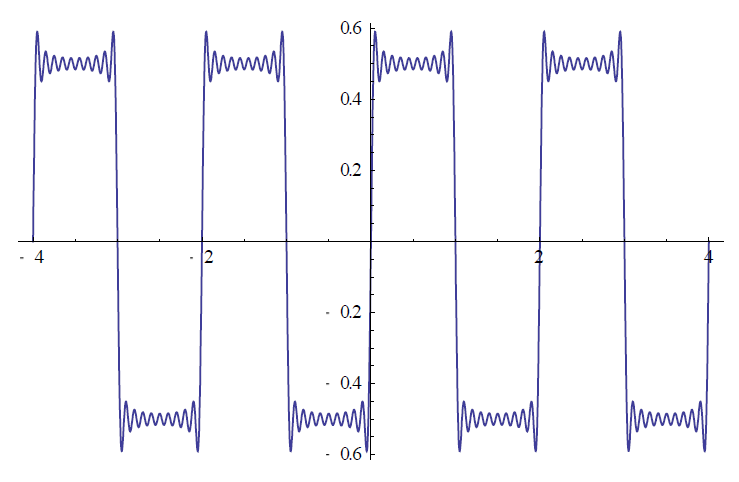
\includegraphics[width=1\linewidth]{5.png}
\end{figure}
And for value 100, we get,
\begin{figure}[H]
	\centering
	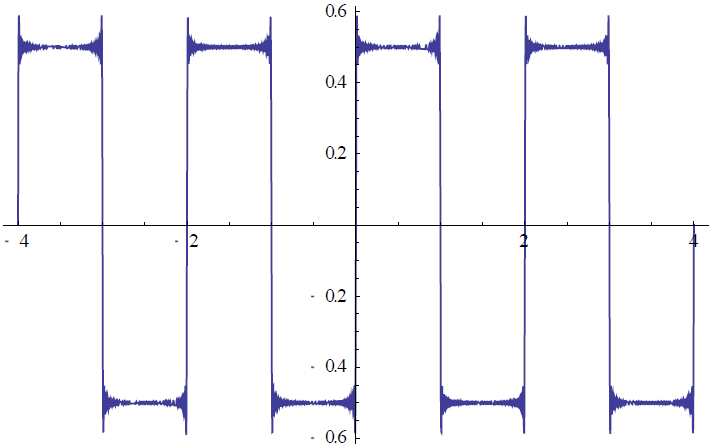
\includegraphics[width=1\linewidth]{6.png}
\end{figure}
\subsection{Four ways to measure the amplitude of a sinusoid}
\begin{enumerate}[a)]
	\item $\rm V_{peak}=V_p=V_{pk}=V_0$ is the peak amplitude of the sinusoid measured in V or mV.
	\item $\rm V_{peak-to-peak}=V_{ppk}=V_{max}-V_{min}=2V_0$ is the value we often use in the lab to determine the overall size of the waveform. We have used it many times in the previous Labs.
	\item $\rm V_{RMS}$ is the Root-Mean-Square, or RMS amplitude of the sinusoid. The sinusoidal voltage $V=V_0\sin(\omega t+\theta)$ dissipates as much power in the load resistor as does the DC voltage equals to $V_{\rm{RMS}}$
	\begin{figure}[H]
		\centering
		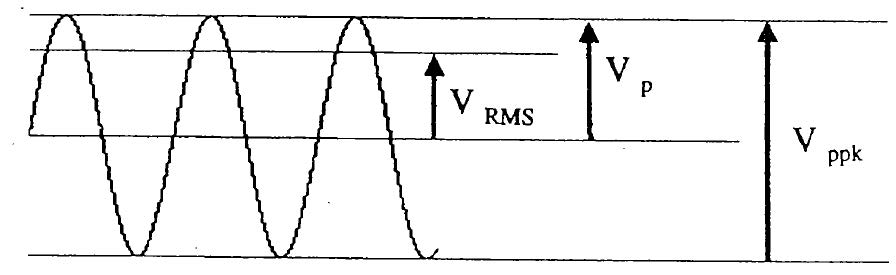
\includegraphics[width=1\linewidth]{7.jpg}
	\end{figure}
    For any periodic function f(t) that has period T, the RMS amplitude is defined as
    $$\rm{Amplitude,RMS}=\sqrt{\frac{1}{T}\int_{t_0}^{t_0+T}f^2(t)dt}$$
    In the case of sinusoid $f(t)=V_0\sin(\omega t+\theta)$,
    $$V_{\rm{RMS}}=\frac{V_0}{\sqrt{2}}=\frac{V_{\rm{peak}}}{\sqrt{2}}=\frac{V_{\rm{ppk}}}{2\sqrt{2}}$$
	\item The above three ways all study the signal in time domain, plotted as voltage vs. time. In this Lab, we also need to study the frequency domain, when you measure their spectra displayed as amplitude vs. frequency. In frequency domain, the oscilloscope measures the amplitude of on a logarithmic scale, using decibels.
    $$\rm Amplitude\ in\ decibels(dBv)=20\log\left(\frac{Amplitude\ in\ V_{RMS}}{1V_{RMS}}\right)$$
    Decibels are used to calculate ratios of two amplitudes on a logarithmic scale.
    $$\rm Ratio,in\ decibels(dB)=20\log\left(\frac{Amplitude\ of\ signal\ \sharp 2,RMS}{Amplitude\ of\ signal\ \sharp 1,RMS}\right)$$
\end{enumerate}
\section{Measurement}
\subsubsection{Part I}
\begin{enumerate}
	\item On the function generator, set a sine wave at 1 [kHz] and keep its amplitude at 3 [Vpp]. The load must be High-Z mode.
	\item Record the parameters on the datasheet. Fill the table with the data set on the function generator and displayed on the oscilloscope.
	\item Repeat the Step 2 with a sine wave at 1.5 [kHz] and 5 [Vpp] on the function generator. The load should remain High-Z mode.
	\item In post-report, calculate the rise time in theory and compare it with the values displayed on the oscilloscope.
	\item Reminder: $\mathrm{RiseTime}=\dfrac{\sin^{-1}(\frac{V_{min}+0.9V_{\rm{pp}}}{0.5V_{\rm{pp}}})-\sin^{-1}(\frac{V_{min}+0.1V_{\rm{pp}}}{0.5V_{\rm{pp}}})}{2\pi f}$
\end{enumerate}
\subsubsection{Part II}
\begin{enumerate}
	\item First, we set a sine wave and a square wave, respectively. The frequency is 1 [kHz] and the amplitude is 3 [Vpp].
	\item On the oscilloscope, set 1 [V/div] and 5 [ms/div].
	\item Push the “MATH” button and select “FFT” function.
	\item Push the “cursor” button and select “trace” mode to trace the spectrum.
	\item When the cursor reach a peak of the spectrum, record the Frequency in [kHz] and the Amplitude in [dBV].
	\item Set another sine wave and a square wave. The frequency is 2 [kHz] and the amplitude is 6 [Vpp]. Repeat the steps above.
	\item In post-report, we need to calculate the theoretical amplitude of sine wave in [dBV]. Besides, you need to calculate the $V_{\rm{peak}}$ of each square wave measured in Part II. We would give a brief conclusion on what we learn from this lab.
	\item Reminder: for sine wave. $\rm{dBV}=20\log(\dfrac{\rm{Amplitude\ in}\ V_{\rm{RMS}}}{1\ V_{\rm{RMS}}})$
	\item Reminder: for square wave. $V_{\rm{peak}}=\sqrt{2}\cdot10^{\frac{\rm{Amplitude\ in\ [\rm{dBV}]}}{20}}$
\end{enumerate}
\section{Results and Calculations}
\subsection{Part I}
\begin{table}[H]
	\centering
	\begin{tabular}{|c|c|c|}
		\hline
		                     & Set on Function Generator & Measured with Oscilloscope \\
		\hline
		Amplitude in Vpp [V] & 3.000                     & 3.14                       \\
		\hline
		Frequency [kHz]      & 1.000000000               & 1.0018                     \\
		\hline
		Rise Time [$\mu$s]   & 295.2                     & 294.7                      \\
		\hline
		Amplitude in Vpp [V] & 5.000                     & 5.11                       \\
		\hline
		Frequency [kHz]      & 1.500000000               & 1.4999                     \\
		\hline
		Rise Time [$\mu$s]   & 196.8                     & 189.5                        \\
		\hline
	\end{tabular}
	\caption{Rise Time Measurement.}
\end{table}
For Vpp of 3V amplitude in the experiment,

$$\mathrm{RiseTime_{exp}}=294.7\,\rm \mu s$$

Theoretically,

$$\mathrm{RiseTime_{theo}}=\dfrac{\sin^{-1}(\frac{V_{min}+0.9V_{\rm{pp}}}{0.5V_{\rm{pp}}})-\sin^{-1}(\frac{V_{min}+0.1V_{\rm{pp}}}{0.5V_{\rm{pp}}})}{2\pi f}=295.2\,\rm \mu s$$

The relative error is $-0.17\%$.

For Vpp of 5V amplitude in the experiment,

$$\mathrm{RiseTime_{exp}}=189.5\,\rm \mu s$$

Theoretically,

$$\mathrm{RiseTime_{theo}}=\dfrac{\sin^{-1}(\frac{V_{min}+0.9V_{\rm{pp}}}{0.5V_{\rm{pp}}})-\sin^{-1}(\frac{V_{min}+0.1V_{\rm{pp}}}{0.5V_{\rm{pp}}})}{2\pi f}=196.8\,\rm \mu s$$

The relative error is $-3.7\%$

We find that these relative errors are small enough.
\subsection{Part 2}
\subsubsection{Set the wave at 3 [Vpp] 1 [kHz]}
\begin{table}[H]
	\centering
	\begin{tabular}{|c|c|c|}
		\hline
		Peak  & Frequency (measured) [kHz] & Amplitude (measured) [dBV] \\
		\hline
		$f_0$ & 1.000000000                & -0.250                       \\
		\hline
	\end{tabular}
	\caption{FFT spectrum for Square Wave.}
\end{table}
$$A_{\rm{dBV,exp}}=-0.25$$

Theoretically,

$$A_{\mathrm{dBV,theo}}=20\log\left(\frac{A_{\mathrm{RMS}}}{1V_{\mathrm{RMS}}}\right)=0.51$$

The relative error is $-149.0\%$
\begin{table}[H]
	\centering
	\begin{tabular}{|c|c|c|}
		\hline
		Peak   & Frequency (measured) [kHz] & Amplitude (measured) [dBV] \\
		\hline
		$f_0$  & 1.000000000                & 1.85                       \\
		\hline
		$3f_0$ & 3.000000000                & -7.70                      \\
		\hline
		$5f_0$ & 5.000000000                & -12.12                     \\
		\hline
		$7f_0$ & 7.000000000                & -15.07                     \\
		\hline
		$9f_0$ & 9.000000000                      & -17.22                     \\
		\hline
	\end{tabular}
	\caption{}
\end{table}
\subsubsection{Set the wave at 6 [Vpp] 2 [kHz]}
\begin{table}[H]
	\centering
	\begin{tabular}{|c|c|c|}
		\hline
		Peak  & Frequency (measured) [kHz] & Amplitude (measured) [dBV] \\
		\hline
		$f_0$ & 2.000000000                & 5.76                       \\
		\hline
	\end{tabular}
	\caption{FFT spectrum for Sine wave.}
\end{table}
In our experiment,

$$A_{dBV}=5.76$$

Theoretically,

$$A_{dBV}=20\log\left(\frac{A_{RMS}}{1V_{RMS}}\right)=6.53$$

The relative error is $-11.8\%$
\begin{table}[H]
	\centering
	\begin{tabular}{|c|c|c|}
		\hline
		Peak   & Frequency (measured) [kHz] & Amplitude (measured) [dBV] \\
		\hline
		$f_0$  & 2.000000000                & 7.85                       \\
		\hline
		$3f_0$ & 6.000000000                & -1.71                      \\
		\hline
		$5f_0$ & 10.000000000               & -6.13                      \\
		\hline
		$7f_0$ & 14.000000000               & -9.09                      \\
		\hline
		$9f_0$ & 18.000000000               & -11.22                     \\
		\hline
	\end{tabular}
	\caption{FFT spectrum for Square wave.}
\end{table}
\begin{figure}[H]
	\centering
	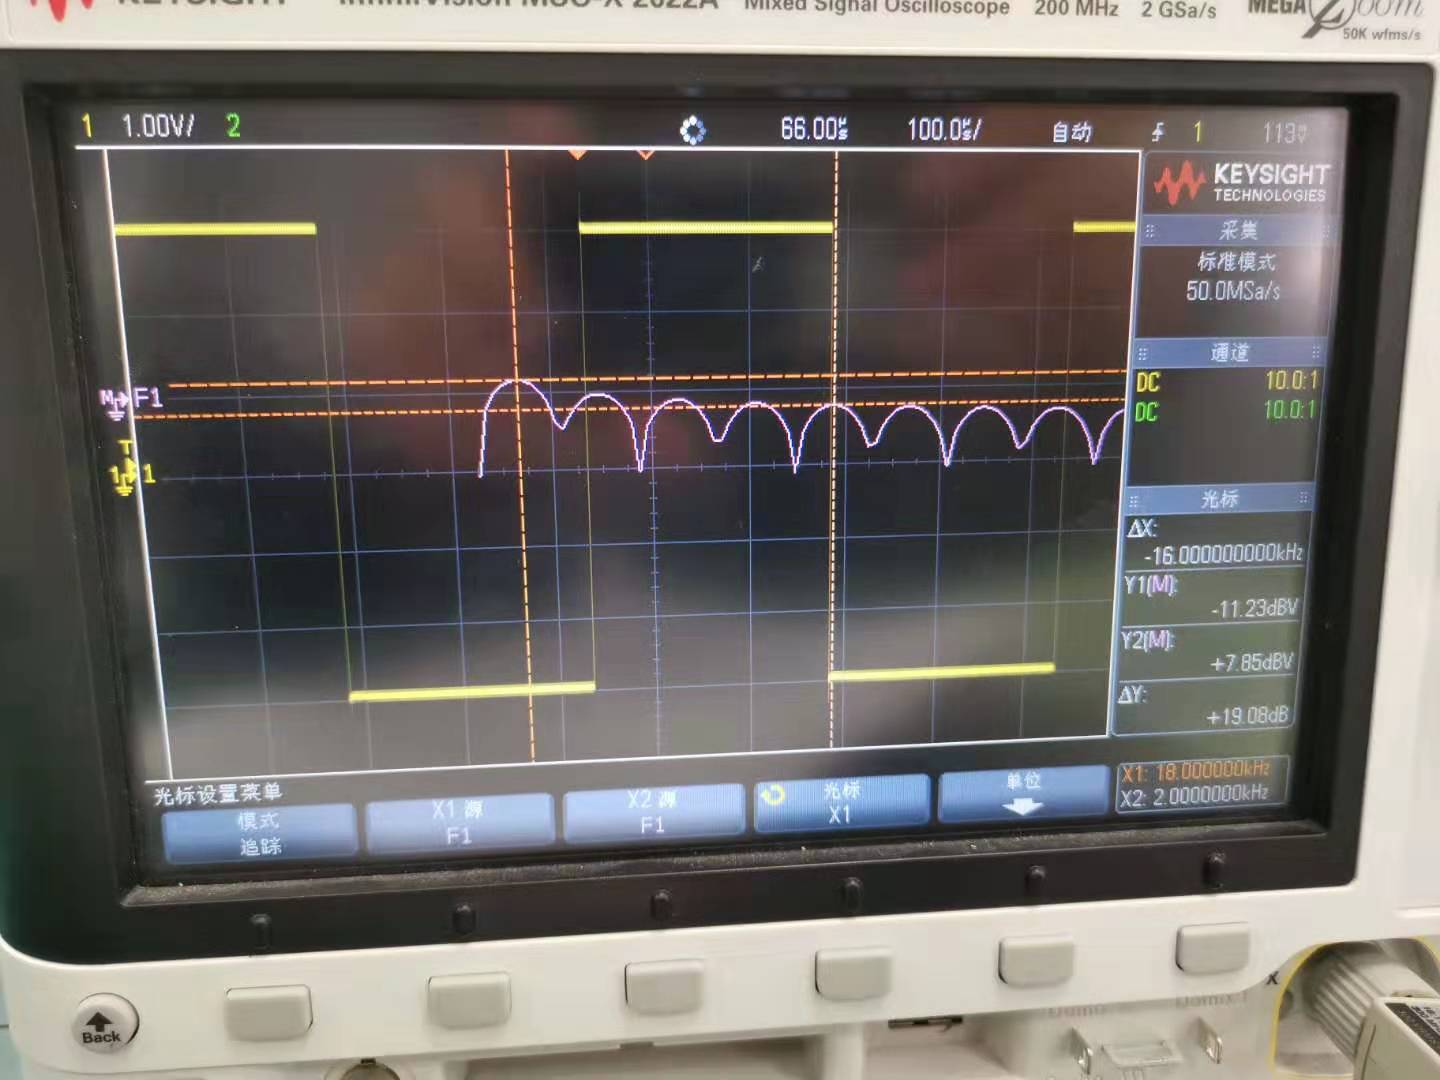
\includegraphics[width=0.8\linewidth]{8.jpg}
\end{figure}
\begin{figure}[H]
	\centering
	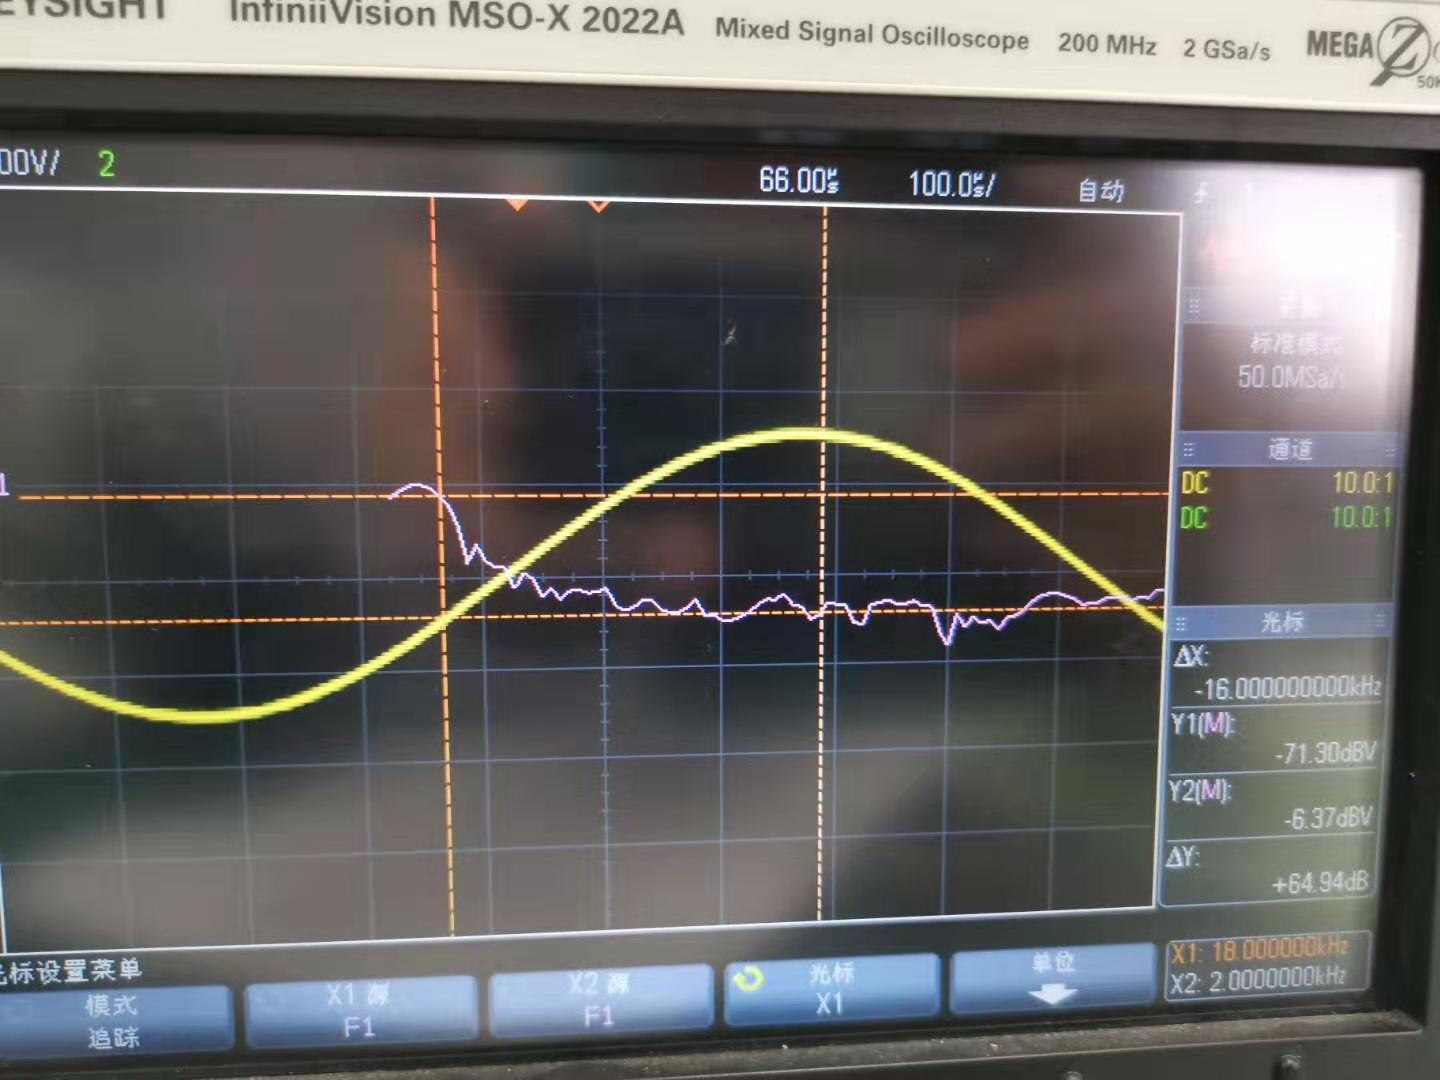
\includegraphics[width=0.8\linewidth]{9.jpg}
\end{figure}
\begin{figure}[H]
	\centering
	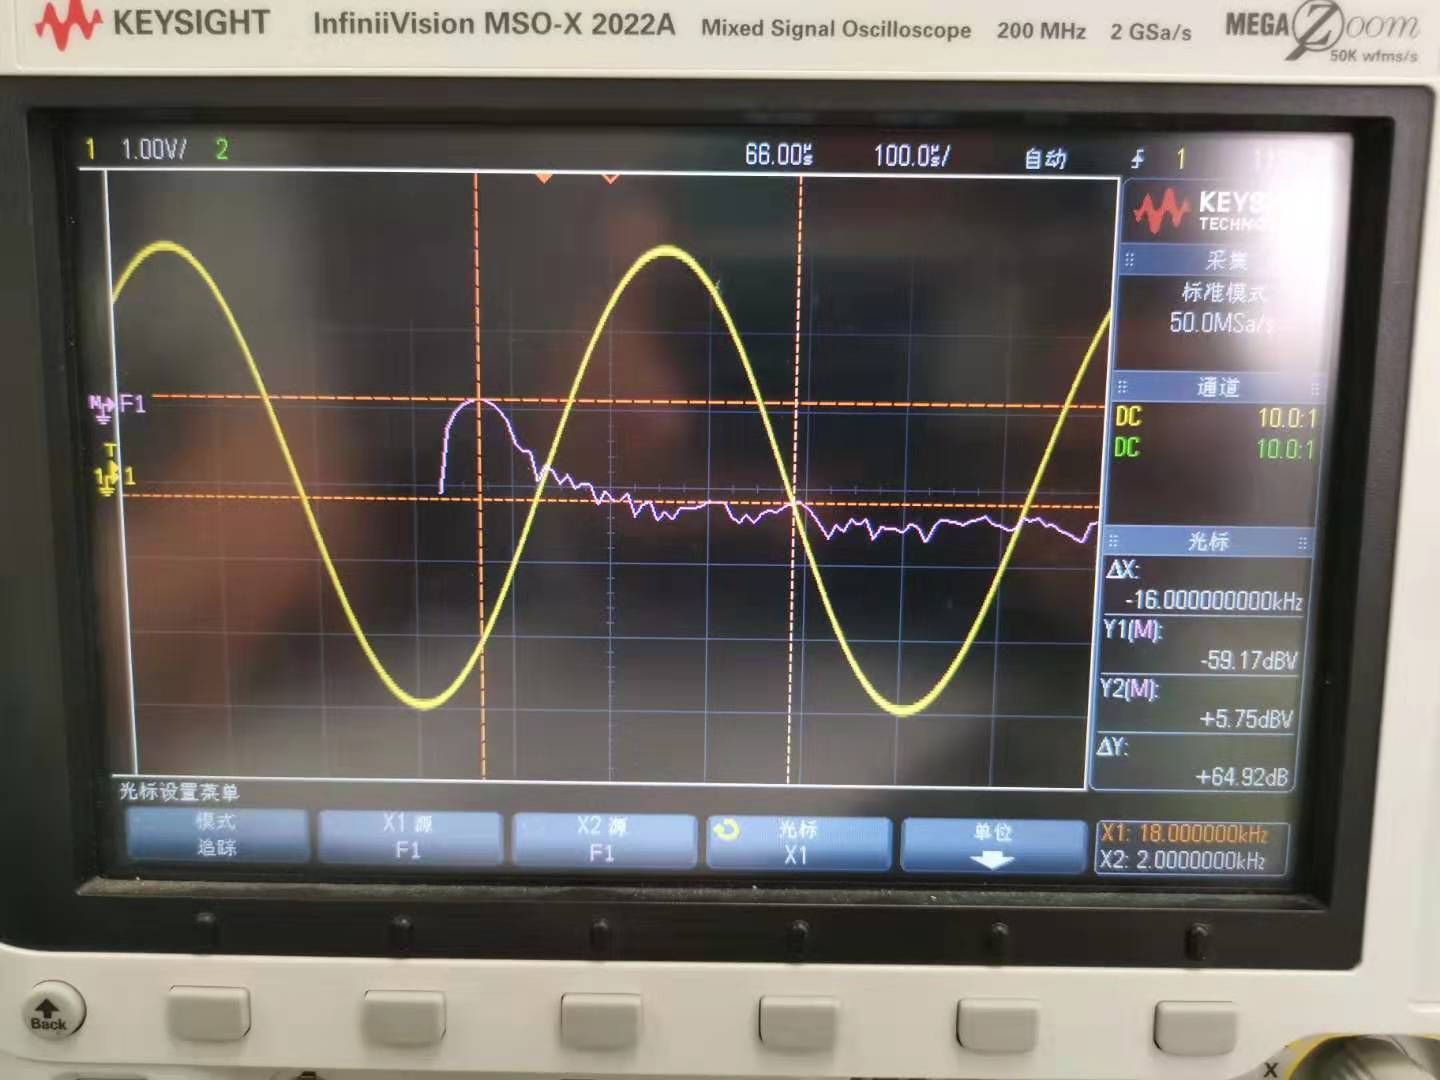
\includegraphics[width=0.8\linewidth]{10.jpg}
\end{figure}
\begin{figure}[H]
	\centering
	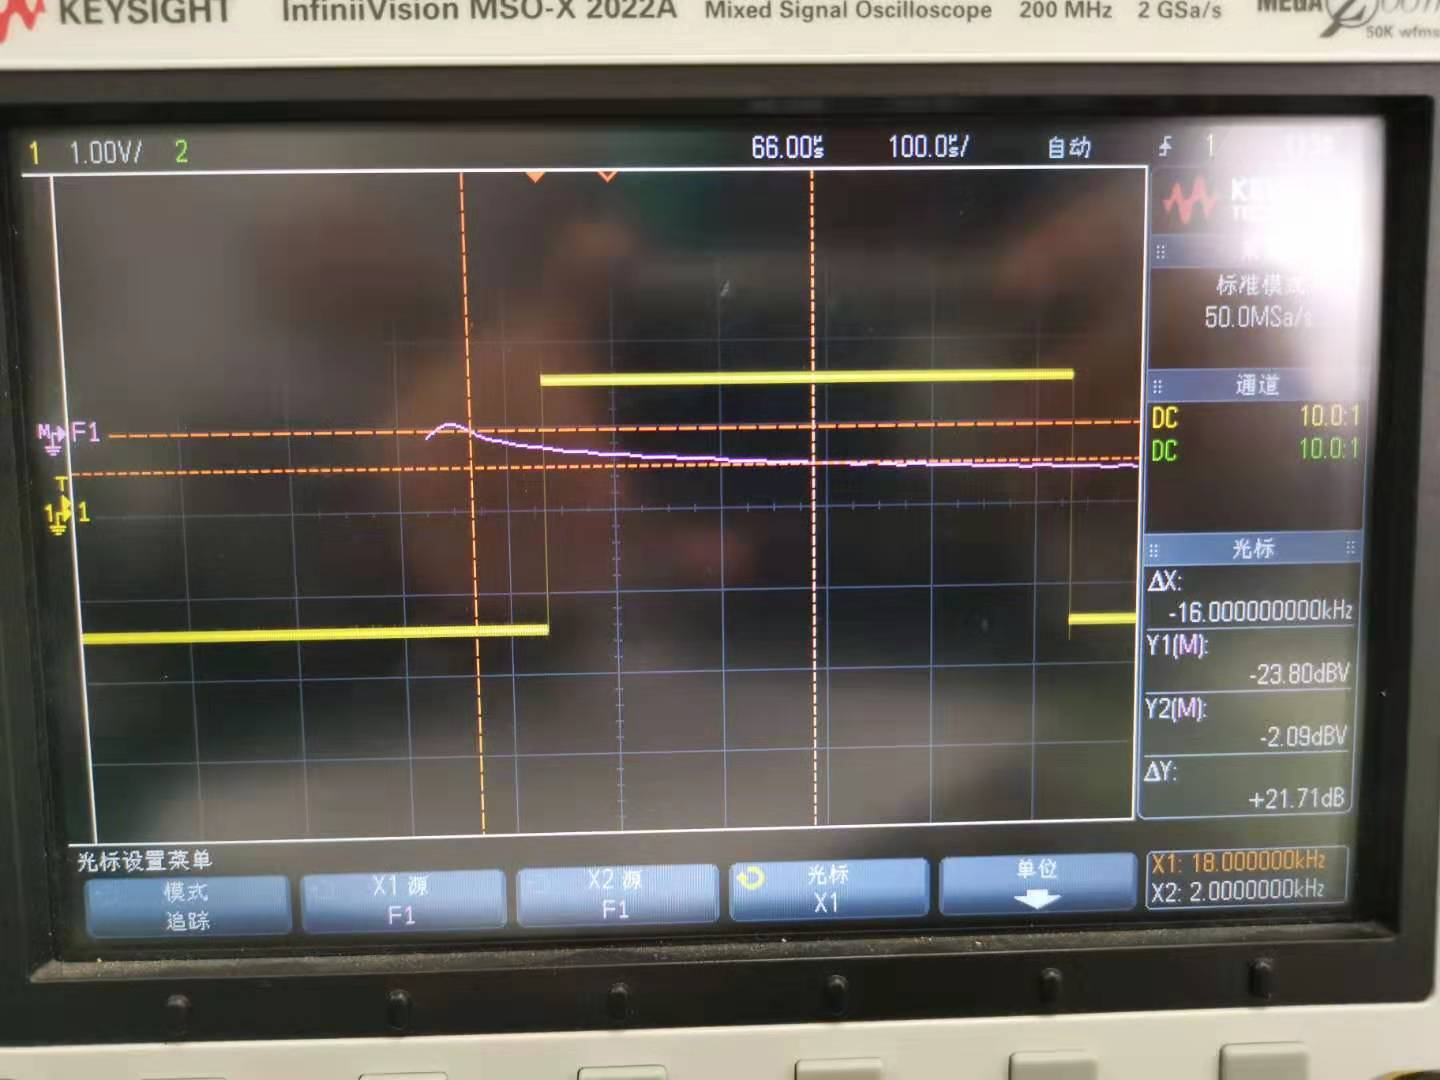
\includegraphics[width=0.8\linewidth]{11.jpg}
\end{figure}
\section{Conclusions and discussion}
In the experiment, we learned how to define, calculate, and measure the amplitude, the Rise Time, and the Fall time of a sinusoidal signal. We learned how to observe FFT spectra of signal on the oscilloscope and measure their parameters by setting cursors. We observed and measured the waveforms and FFT spectra of various signals. From the results, we compared the theoretical results obtained in the Pre-Lab with the experimental In-Lab data.

For Part I, the relative errors are quite small, but in Part II, the relative errors are quite large. One of the reasons might be that the amplitudes were measured in [dBV] that is a logarithm, which will vary a lot near 0 in a small range. On the other hand, the machines are not stable, so that the same parameters would produce different measurements and calculation results.
\section*{Reference}
\begin{hangparas}{2em}{1}
Ve215 Fall 2016 Lab 4 AC Lab Manual.

Circuits make sense A new Lab Book for introductory Course In Electric Circuits. Fifth edition. Alexander Ganago.
\end{hangparas}
\vspace{17cm}
\section*{Data sheet}
\end{document}